\documentclass[tikz,border=8pt]{standalone}
\usepackage[T1]{fontenc}
\usepackage{tikz}
\usetikzlibrary{arrows.meta,positioning,fit,backgrounds}

\begin{document}
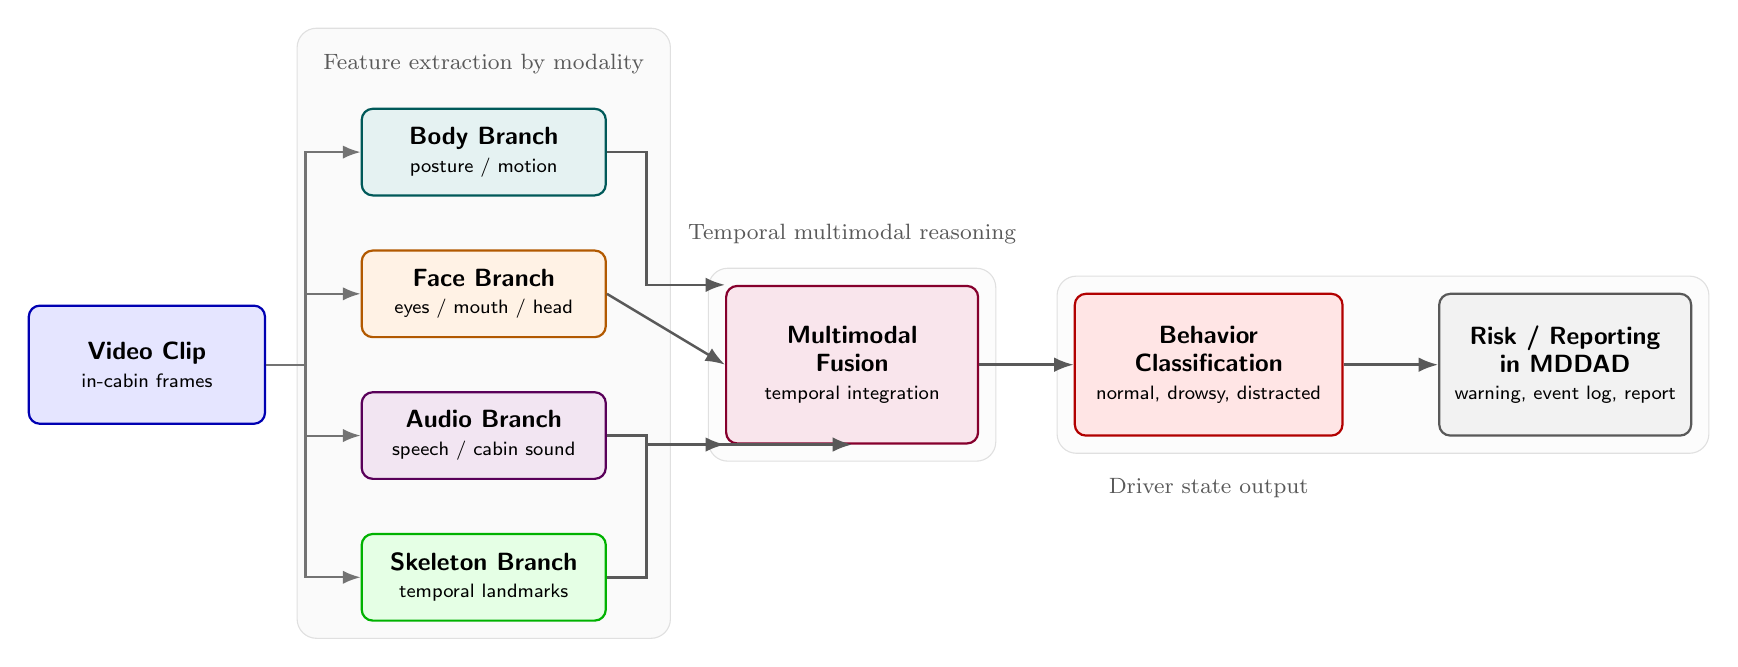
\begin{tikzpicture}[
  font=\sffamily\small,
  >=Latex,
  node distance=8mm and 10mm,
  box/.style={
    draw=#1!70!black,
    fill=#1!10,
    rounded corners=4pt,
    line width=0.8pt,
    align=center,
    minimum height=13mm,
    minimum width=28mm,
    inner sep=4pt
  },
  smallbox/.style={
    draw=#1!70!black,
    fill=#1!10,
    rounded corners=4pt,
    line width=0.8pt,
    align=center,
    minimum height=11mm,
    minimum width=31mm,
    inner sep=3.5pt
  },
  arrow/.style={->, line width=0.9pt, draw=black!65},
  brancharrow/.style={->, line width=0.75pt, draw=black!55},
  note/.style={font=\footnotesize, text=black!65, align=center}
]

\node[box=blue, minimum width=30mm, minimum height=15mm] (video) {
  \textbf{Video Clip}\\[-1pt]
  \scriptsize in-cabin frames
};

\node[smallbox=teal, right=12mm of video, yshift=27mm] (body) {
  \textbf{Body Branch}\\[-1pt]
  \scriptsize posture / motion
};
\node[smallbox=orange, right=12mm of video, yshift=9mm] (face) {
  \textbf{Face Branch}\\[-1pt]
  \scriptsize eyes / mouth / head
};
\node[smallbox=violet, right=12mm of video, yshift=-9mm] (audio) {
  \textbf{Audio Branch}\\[-1pt]
  \scriptsize speech / cabin sound
};
\node[smallbox=green, right=12mm of video, yshift=-27mm] (skeleton) {
  \textbf{Skeleton Branch}\\[-1pt]
  \scriptsize temporal landmarks
};

\node[box=purple, right=15mm of face, yshift=-9mm, minimum width=32mm, minimum height=20mm] (fusion) {
  \textbf{Multimodal}\\[-1pt]
  \textbf{Fusion}\\[-1pt]
  \scriptsize temporal integration
};

\node[box=red, right=12mm of fusion, minimum width=34mm, minimum height=18mm] (behavior) {
  \textbf{Behavior}\\[-1pt]
  \textbf{Classification}\\[-1pt]
  \scriptsize normal, drowsy, distracted
};

\node[box=gray, right=12mm of behavior, minimum width=32mm, minimum height=18mm] (mddad) {
  \textbf{Risk / Reporting}\\[-1pt]
  \textbf{in MDDAD}\\[-1pt]
  \scriptsize warning, event log, report
};

\draw[brancharrow] (video.east) -- ++(5mm,0) |- (body.west);
\draw[brancharrow] (video.east) -- ++(5mm,0) |- (face.west);
\draw[brancharrow] (video.east) -- ++(5mm,0) |- (audio.west);
\draw[brancharrow] (video.east) -- ++(5mm,0) |- (skeleton.west);

\draw[arrow] (body.east) -- ++(5mm,0) |- (fusion.north west);
\draw[arrow] (face.east) -- (fusion.west);
\draw[arrow] (audio.east) -- ++(5mm,0) |- (fusion.south west);
\draw[arrow] (skeleton.east) -- ++(5mm,0) |- (fusion.south);

\draw[arrow] (fusion.east) -- (behavior.west);
\draw[arrow] (behavior.east) -- (mddad.west);

\node[note, above=3mm of body] (modalities) {Feature extraction by modality};
\node[note, above=4mm of fusion] {Temporal multimodal reasoning};
\node[note, below=4mm of behavior] {Driver state output};

\begin{scope}[on background layer]
  \node[draw=black!12, fill=black!2, rounded corners=7pt, fit=(body)(face)(audio)(skeleton)(modalities), inner sep=6pt] {};
  \node[draw=black!12, fill=black!1, rounded corners=7pt, fit=(fusion), inner sep=6pt] {};
  \node[draw=black!12, fill=black!1, rounded corners=7pt, fit=(behavior)(mddad), inner sep=6pt] {};
\end{scope}

\end{tikzpicture}
\end{document}
